\documentclass{report}

\usepackage[margin=1in]{geometry}
\usepackage{amsmath,amssymb}
%\usepackage{dsfont} %install texlive-fonts-extra 
\usepackage{tikz}
\usetikzlibrary{bayesnet}
\usepackage{setspace}
\usepackage{xcolor}

\author{Otto Fabius}
\title{SGVB Topic Modeling}
\begin{document}
\large
\doublespacing
\maketitle
\begin{abstract}
	content...
\end{abstract}
\chapter*{}
\onehalfspacing
\section*{List of Symbols}
We use lowercase bold-faced symbols to denote vectors, and uppercase bold-faced symbols to denote matrices. \\ \\
\begin{tabular}{r l}
	\hspace{15mm} $\mathbf{x}$ & Data point \\
	$\mathbf{\hat{x}}$ & Data point normalized to have unit length \\	
	$\theta$ &  Model parameters \\
	$\phi$ & Parameters of approximate posterior model \\
	$z$ & Stochastic latent variable\\
	$\mu$ & Mean of stochastic latent variable\\
	$\sigma ^2 $ & Variance of stochastic latent variable \\
	$\mathcal{L}$ & Lower Bound \\
	$\tilde{\mathcal{L}}$ & Lower Bound estimate\\
	$\tilde{\mathcal{L}_w}$ & Per-word lower bound estimate \\
	$D_{KL}$ & Kullback-Leibler Divergence \\
	$V$ & Number of unique words in a dataset. \\
	$N_d$ & Number of documents in a dataset. \\
	$F$ & Matrix of node feature vectors
\end{tabular}
\\ \\
 We use index $i$ to indicate a data point, index $k$ to indicate a feature, and index $j$ to indicate a latent variable. In all applications in this thesis, our data points are documents represented by count vectors. Therefore, for example, $\mathbf{\hat{x}}_{ik}$ is the relative frequency of word $k$ in document $i$.
\section*{List of Abbreviations}
\begin{tabular}{r l}
	\hspace{10mm} BoW & Bag-of-Words \\
	DEF & Deep Exponential Families \\
	GCE & Graph Convolutional Encoder \\
	LDA & Latent Dirichlet Allocation \\
	SGVB & Stochastic Gradient Variational Bayes \\
	VAE & Variational Autoencoder \\
\end{tabular}

\tableofcontents

\doublespacing
\chapter{Introduction}
Aim, scope and structure of the thesis. 
\section{Research question}
Explain that we want to use sgvb for topic modelling. Introduce research question:
Can we perform large-scale, efficient, high-quality inference on bag-of-words representations of documents with sgvb? \\
Briefly discuss the advantages of this approach compared to other methods in topic modelling (one paragraph)
-	How do we deal with large vocabulary size?\\
-	What consequences do sparsity have/how can they be overcome? \\
-	What is learned in the (continuous) latent representation?



\pagebreak 
\nocite{*}
\bibliographystyle{amsplain}

\chapter{Background}
\section{Variational Inference}
\begin{itemize}
	\item Variational Optimization key idea
	\item Often used for inference problems, decompose the log marginal according to Bishop (eq 10.2)
	\item 
\end{itemize}
Variational Inference methods in general are used when data $\mathbf{X}$ is assumed to be generated through some process from an underlying set of stochastic latent variables $\mathbf{Z}$. The probability of data is therefore modeled as $p(\mathbf{X}) = p(\mathbf{Z}|\mathbf{X})p(\mathbf{Z})$. Moreover, this set of methods is used when the true posterior $p(Z|X)$ can not be evaluated analytically. Variational Bayes introduces a tractable distribution $q(\mathbf{\mathbf{Z}|\mathbf{X}})$ as an approximation to $p(\mathbf{Z}|\mathbf{X}))$.
\\
More on Variational Inference....
\section{Bag-of-words Topic Modelling}

\subsection{LSI and pLSI}
\subsection{LDA}
Explain LDA following (p)LSI and Variational Inference.
\subsection{Deep Exponential Families}

Deep exponential families is relevant for this work for two reasons: It shows that deeper models can be more powerful than LDA, and is currently the state of the art. Nothing in our methods depends on this section.


\section{SGVB}\label{sgvb_section}

Discuss requirements of problem scenario for SGVB to be applicable. \\

Notes:\\
- No simplifying assumptions are made about the marginal or posterior probabilities, as is the case in other VB methods (check!!) \\
- $q(\mathbf{Z}|\mathbf{X})$ is not necessarily factorial and its parameters $\phi$ are not computed from some closed-form expectation (as in mean field VI)
- General purpose introduction of sgvb . \\

- areas of success of sgvb.

\section{Stick-Breaking VAE}\label{sbvae_section}
	As detailed in \ref{sgvb_section}, one restriction of SGVB in general is the need for a differentiable, non-centered parametrization of the latent variables. Therefore, e.g. Beta distributed latent variables (as used in e.g. LDA \cite{bleil2003latent}), can not be used in the SGVB framework. \\ Nalisnyck \& Smith extend SGVB to Stick-breaking priors by using the Kumaraswami Distribution as the approximate posterior. The rest of this section \ref{sbvae_section} is not much more than a description of the relevant part of Nalisnyck \& Smyth \cite{nalisnick2016deep}.
\subsection{Stick-breaking Priors}
\subsection{Kumaraswami Distribution} 
\subsection{SGVB with Stick-Breaking Priors}

\section{Graph Convolutional Networks}\label{GCN_section}
Note that this is only relevant for one of our models. Describe Kipf and Welling paper.
\chapter{SGVB Topic Models}
\section{Introduction}
In this Chapter, we present in detail the models we use in our experiments. 

\section{Topic VAE}

In this section we describe our initial approach for topic modeling with SGVB. It does not deviate conceptually from the VAE model used in the experiments by Kingma and Welling\cite{kingma2013auto}, so one might call this a Topic VAE. We will describe the application-specific choices made within the general SGVB framework as described in section \ref{sgvb_section}, and derive the objective function used for optimization. 

\subsection{Model Specifics}

Within the general SGVB framework described in the previous chapter, we specify the following characteristics of our VAE Topic model:

\begin{enumerate}
	\item The representation of our documents $\mathbf{X}$
	\item The encoder $q(\mathbf{z}|\mathbf{x})$
	\item $p(z)$, a prior  over the latent variables
	\item The transformation function $g_\phi(\boldsymbol{\epsilon},\mathbf{x})$
	\item The  probability distribution  $p(\mathbf{\epsilon})$ from which to draw $\epsilon \sim p(\epsilon)$
	\item The decoder $p(\mathbf{x}|\mathbf{z})$
\end{enumerate}

The representation of the documents is a normalized Bag-of-Words representation s.t. document $i$ is represented by a unit vector $\hat{\mathbf{x}_i} = \frac{\mathbf{x}_i}{\sum_{k=1}^{V}x_{ik}}$. Although normalizing data is standard practice in neural network approaches (references...), typically each feature is normalized separately. In our approach, however, all features (word counts) of a data point (document) are normalized s.t. they represent word probabilities. This representation no longer contains information on the length of documents, which arguably weakly relates to topics.
\\
The encoder $q(\mathbf{z}|\mathbf{x})$ is a fully connected neural network with one or more hidden layers with ReLu activation functions. The input is $\mathbf{d}$ and the output is the mean and log standard deviation \{$\boldsymbol{\mu}, \log \boldsymbol{\sigma} ^2\}$ of the Multivariate Gaussian $N(\boldsymbol{\mu}, \boldsymbol{\sigma} ^2\textbf{I})$. For one hidden layer this would be the following function:
\begin{align}
\mathbf{h_{e1}} = \text{ReLu}(\mathbf{\hat{x}}\mathbf{W_{e1}} + \mathbf{b}) \\
\boldsymbol{\mu} = \mathbf{h_{e1}W}_{\mu} \\
\log \boldsymbol{\sigma}^2 = \mathbf{h_{e1}W}_{\sigma}
\end{align} 
We use prior $p(z) = N(0,\textbf{I})$
\\
Our encoder and prior are identical to the experiments in \cite{kingma2013auto}, and so ar our transformation function $g_\phi(\boldsymbol{\epsilon},\mathbf{x}) = \boldsymbol{\mu} + \boldsymbol{\sigma}^2\odot \boldsymbol{\epsilon}$, and sampling function $p(\epsilon) = N(0,\textbf{I})$. Note that throughout this work we consistently only use one sample $\epsilon$ for each latent representation $\mathbf{z}$, and we therefore do not use an index for this.\\
The decoder $p(\mathbf{x}|\mathbf{z})$ is also a neural network with as input (a sample from) latent representation $\mathbf{z}$ and as output the probabilities of a Multinomial distribution, with a ReLu activation function used in each hidden layer. With one hidden layer, this would specified by:

\begin{align}
\mathbf{h_{d1}} = \text{ReLu}(\mathbf{zW_{d1}+b_{d1}})
\\
p(\mathbf{x}|\mathbf{z}) = \text{softmax} (\mathbf{h_{d1}W_{d2}}+\mathbf{b_{d2}})
\end{align}
Where the $\text{softmax}(\mathbf{x}) = \dfrac{e^{\mathbf{x}}}{\sum_{k=1}^{K}e^{x_k}}$


Discuss implications of plate difference? Discuss alternative approach with separate latent variables and/or noise for each word?\\ \\

\subsection{Objective Function}
The general form of the SGVB estimator is:

\begin{align}
\tilde{\mathcal{L}}(\boldsymbol{\theta}, \boldsymbol{\phi}, \mathbf{x_i}) = -D_{KL}(q_\phi (\mathbf{z}|\mathbf{x}_i)||p(_\theta(\mathbf{z}))  + \frac{1}{L}\sum_{l=1}^{L}\log p_\theta(\mathbf{x}_i|\mathbf{z}_i)
\end{align}

And because we consistently only use one sample from $p(\boldsymbol{\epsilon})$ per data point, this simplifies to:

\begin{align}
\tilde{\mathcal{L}}(\boldsymbol{\theta}, \boldsymbol{\phi}, \mathbf{x_i}) = -D_{KL}(q_\phi (\mathbf{z}|\mathbf{x}_i)||p(_\theta(\mathbf{z}))  + \log p_\theta(\mathbf{x}_i|\mathbf{z}_i)
\end{align}

Because we use Gaussian latent variables with diagonal covariance, we can integrate the KL Divergence analytically as done in Kingma and Welling \cite{kingma2013auto}. \textit{Might need to elaborate on this, if not already done so in the background chapter}. Adding the expression for the Multinomial likelihood $p_\theta(\mathbf{x}_i|\mathbf{z}_i)$, we then have
\begin{align}\label{LBest}
\tilde{\mathcal{L}}(\boldsymbol{\theta}, \boldsymbol{\phi}, \mathbf{x_i}) = - \frac{1}{2}\sum\limits_{j=1}^{J}\{1+\log \sigma_{\phi ,ij}^2 - \mu_{\phi,ij}^2 - \sigma_{\phi ,ij}^2\}  + 
\sum_{k=1}^K x_{ik} \log (y_{ik})
\end{align}
\\
Notably, this is the lower bound per \textit{document}. In (bag-of-words) topic modeling, likelihood measures such as perplexity are usually per-word measures. To obtain a per-word lower bound, we must divide the total lower bound for a set of evaluated documents by the number of words in that set: 
\begin{align}\label{perwordLBest}
\tilde{\mathcal{L}_w}(\boldsymbol{\theta}, \boldsymbol{\phi}, \mathbf{X}) = \frac{1}{\sum\limits_{i=1}^{N}\sum\limits_{k=1}^{K}\mathbf{X}_{ik}}\sum\limits_{i=1}^N \tilde{\mathcal{L}}(\boldsymbol{\theta}, \boldsymbol{\phi}, \mathbf{x_i})
\end{align}

We cannot compare this lower bound estimate in \ref{perwordLBest} nor the one in \ref{LBest} directly to different models or measures and the lower bound estimate is therefore merely for model optimization. Although \ref{LBest} and \ref{perwordLBest} are functionally equivalent, a per-word lower bound is independent of average document size and more relatable to other per-word measures in topic modeling, so we prefer to use this measure when reporting experimental results over e.g. the lower bound per document.



\section{Stick Breaking Topic VAE}
 as described in this thesis, is that it assumes the latent variables are (approximately) normally distributed. For some datasets, it might be hard to encode data points in multiple independent normally distributed variables. LDA, with it's binary latent variables, has a much more discriminative distribution (the Beta Distribution) over latent variables non-centered distribution, such as in many binary latent variable models (e.g. LDA) might be might be more discriminative. As we have sparse data where data points (i.e. documents) frequently can be described by only a few of the used latent variables (roughly corresponding to topics), this seems particularly applicable to our application.  \\
Therefore, we also investigate the use of a Stick-Breaking VAE (Nalisnyck \& Smith \cite{Nalisnick2016deep}) for Topic Modelling\\
For $a = 1$ or $b = 1$, Kumaraswami equals Beta.

\subsection{Stick Breaking Priors}

For now, see SVBAE 4.1

\subsection{Reparametrization}

\subsection{KL Divergence}

We need the KL divergence between the Kumaraswami posterior and the Dirichlet prior:

\begin{align}
KL(q(\mathbf{\mathbf{\pi}_i}|\mathbf{x}_i)||p(\mathbf{\pi}_i;\alpha_0)) = \sum_{k=1}^{K}\mathbb{E}_q [\log q(v_{i,k})] - \mathbb{E}_q \log p(v_{i,k})]
\end{align}

Truncating the infinite-dimensional distribution (sti8ck breaking process) by setting $\pi_i,K$ to s.t. $\sum_{k=1}^{K}\pi_{i,k} = 1$, the KL divergence can be written as:

\begin{align*}
\sum_{k=1}^{K}\mathbb{E}_q [\log q(v_{i,k})] - \mathbb{E}_q \log p(v_{i,k})] = \frac{a_0 -\alpha}{a_0}(-e-\Psi(b_\phi-\frac{1}{b_\phi}))+ \log(a_\phi b_\phi) + \log B(\alpha, \beta) \\
- \frac{b_\phi -1}{b_\phi} 
+ (\beta-1)b_\phi\sum_{m=1}^{\infty}\frac{1}{m+a_\phi b_\phi}B(\frac{m}{a_\phi},b_\phi)
\end{align*}

(is the Digamma function differentiable? If so, how to implement? Currently 2nd order taylor which works fine)\\

where $e$ is Euler’s constant, $\Psi(\cdot)$ is the Digamma function, and $B(\cdot)$ is the Beta function.
The infinite sum, which originates from a Taylor appriximation, can be approximated well by the first 2 or 3 terms. When $\beta$ is one, as when using a weighted sum of Beta distributed latent variables for a Dirichlet distribution, this last term vanishes. For a full derivation see Nalisnyck and Smith, SB-VAE.



\section{Random Projections}
Idea: use a random projection of all scarce words in the dataset as extra information for the encoder. This hardly adds computational complexity, but might still improve inference.

\section{Graph Convolutions for Topic VAE}

Bag-of-words data can be seen as a bi-partite graph between document nodes and word nodes (add image of this graph?). From this perspective, it makes sense to look into incorporating the work by Kipf \& Welling on Graph Convolutional Networks in our approach. \\
As detailed in \ref{GCN_section}, the first layer of a GCN is given by:
\begin{align}\label{GCE_layer}
H = \text{ReLU}(\bar{D}^{-\frac{1}{2}}\bar{A}\bar{D}^{-\frac{1}{2}}FW)
\end{align}
\\
Where ReLU can be an other nonlinearity of choice. $\bar{A}$ is the (symmetric) adjacency matrix $A$ with added self connections $I$:$\bar{A} = A+I$, and $\bar{D_{ii}}=\sum_j\bar{A}_{ij}$. Further, $W$ is a trainable weight matrix similar to those in our earlier approaches. In our application, $\bar{A}$ would be of dimension $(N_d + V) \text{ x } (N_d + V)$, with both the upper left corner and the bottom right corner an identity matrix (note: explain what $A_{ij}$ is). We can rewrite \ref{GCE_layer} as:

\begin{align}\label{GCE_layer}
H = \text{ReLU}(X'W)
\end{align}

Where $X' = \bar{D}^{-\frac{1}{2}}\bar{A}\bar{D}^{-\frac{1}{2}}F$. A straightforward way of using Graph Convolutions is to incorporate one (or more) Graph Convolutions in our encoder as in \ref{GCE_layer}. \\ In this case, $F$ would logically reduce to $I$ since we have no node features. \\
Let us rewrite $X'W$, leaving out the self-connections $\mathbf{I}$ in $\mathbf{A}$: 
\begin{align}
X' = \bar{D}^{-\frac{1}{2}}
\left( \begin{matrix} 
0 && G \\
G^T && 0
\end{matrix} \right) \bar{D}^{-\frac{1}{2}}W = \\
\left(\begin{matrix}
\bar{G}W_1 \\
\bar{G^T}W_2
\end{matrix}\right)\label{highlow}  
\end{align}
Where $\bar{G}_{ij} = 
\frac{G_{ij}}{\sqrt{\sum_i G_{ij} \sum_{j} G_{ij}}}$ \textit{indexing isnt correct yet I think}.

We now have multiplications with two weight matrices $W_1$ and $W_2$, one that has parameters for each $N_d$ documents and one that has parameters for each word in $V$. Having parameters for each document is not scalable to large datasets, especially since a batched approach to $\bar{G^T}W_2$ is impossible.\\
One way of encoding some document-level information is to use the covariance matrix $\bar{G^T}\bar{G}$ in stead of $\bar{G^T}$. Now, the number of parameters in our first layer would scale with $(2\cdot V)$ instead of $(V+N)$. \ref{highlow} now becomes:
\\
\begin{align}
\left(\begin{matrix}
\bar{G}W_1 \\
\bar{G^T}\bar{G}W_c
\end{matrix}\right)
\end{align}
\\
Using a minibatch approach to $\bar{G^T}\bar{G}W_2$ requires calculating $\bar{G^T}\bar{G_{batch}}W_c$ for each batch, which is of complexity $O(V\text{ x }V \text{ x } h)$, where $h$ is the number of hidden units. Even for a large batch size, this is much more expensive than calculating the sparse multiplication $\bar{G}_{batch}W_1$, which is of $O(\text{nonzero}(\bar{G}_{batch}) \text{ x } h \text{ x } \text{batchsize})$. 
\\
Using the full covariance matrix for each minibatch allows for computing $\bar{G^T}\bar{G}$ only once. However, writing out the first layer for one row $\mathbf{g}$ of $\bar{G}$ shows us this approach does not combine information in $\mathbf{g}$ and $\bar{G}_T\bar{G}$:
\begin{align}
h_1 = \text{ReLU}(
\left(\begin{matrix}
\mathbf{g} \\
\bar{G^T}\bar{G}
\end{matrix}\right)W_1 +b_1)
\\
h_1 = 
\text{ReLU}(\left(\begin{matrix}
	\mathbf{g}W_{1a} \\
	\bar{G^T}\bar{G}W_{1b}
\end{matrix}\right) + b_1)
\end{align}
\\
Note that leaving out $\bar{G}^TW_2$ in \ref{highlow} leaves us with the original first layer of our encoder, except with a different TF-IDF-like normalization of our data. While this insight perhaps does not change our model much, it is worth some experiments, which we will detail in Chapter \ref{experiments}   \textit{Write out this normalization and forecast experiments.} 
\chapter{Experiments and Results}\label{experiments}
\section{General}
First we will describe the datasets used, discuss briefly the evaluation metrics reported, as well as describe the general optimization method used in our experiments.
	\subsection{Datasets}\label{datasets}
	For all methods, we ran experiments on the KOS and NY Times datasets, freely available at UCI\footnote{https://archive.ics.uci.edu/ml/datasets/Bag+of+Words}. Both datasets contain only words that occur more than ten times in the whole dataset. The KOS dataset contains 3430 documents and has a vocabulary size of 6906. The dataset was split into 3300 training documents and 130 test documents. The NY times dataset consists of 300,000 documents and has a vocabulary size of 102,660 words. For the NY Times dataset, we only use words that occur over 3,000 times in the dataset, which are 5319 unique words. This makes training time and model evaluation a lot faster, as both scale approximately linearly with input dimensionality. \textit{Leaving out infrequent words only has a minor effect on the perplexity of bag-of-word topic model perplexity, mainly due to Zipf's law (Cite Kobayashi).} For this dataset, a test set of 1,000 documents was used.
	\\
	\subsection{Evaluation}
	
	Evaluating Topic models is often done by calculating the perplexity of held out words on the test set (e.g. \cite{blei2003latent, newman2007distributed, ranganath2015deep}). In this work, held-out perplexity is calculated for the test set as in Newman \& Welling \cite{newman2007distributed} by using half the words, randomly sampled, in each document for inference (i.e. calculating $p(\mathbf{z}|\mathbf{x})$ ). Let $\mathbf{x}_{i}^{(s)}$ be the half of document $\mathbf{x}_i$ used for inference, and $\mathbf{x}_{i}^{(u)}$ be the other half of the document, used for evaluation. The average per-word perplexity of the unseen words $\mathbf{X^{(u)}}$ in the test documents $X$ under the word-probabilities $p(X|Z)$, where $Z^s \sim p(\mathbf{Z}|X^{(s)})$ is then given by:
	
	
	\begin{align}
	\text{perplexity} =  \frac{1}{\sum\limits_{i=1}^{N}\sum\limits_{k=1}^{K}x_{ik}}\sum\limits_{i=1}^N\sum\limits_{k=1}^{K} \log p(x_{k}|\mathbf{z}_{i}^{s})x_{ik}^{u}
	\end{align}\\
	\textit{Note: take another look at perplexity calculation in DEF}
	\\
	Add some stuff on reporting the lower bound. Refer to earlier elaboration on LB per word.
	
	\subsection{General Optimization Method}\label{optim_section}
	We use Adam, learning rate 0.003 unless otherwise stated. Batch size 50 for KOS and 200 for NY Times. Describe weights initialization. KL Divergence is linearly increased during first 100 epochs of training. (different for NY Times?).
	

	\section{Experiments}
	\subsection{Topic VAE}
	
	From Hinton: 24.12 \textit{A recipe for choosing the number of hidden units
		Assuming that the main issue is overfitting rather than the amount of computation at training or
		test time, estimate how many bits it would take to describe each data-vector if you were using a good
		model (i.e. estimate the typical negative log2 probability of a data vector under a good model). Then
		multiply that estimate by the number of training cases and use a number of parameters that is about
		an order of magnitude smaller. If you are using a sparsity target that is very small, you may be able
		to use more hidden units. If the training cases are highly redundant, as they typically will be for very
		big training sets, you need to use fewer parameters.}\\

	In this section we outline our experiments with the VAE Topic Model. \textit{(brief summary of section?)} 
	
	
	
	\subsubsection{Experiment 1: A First Model}
	Describe choice of number of latent variables, hidden units to start with (200e, 20d). Report lower bound train and test over time, as well as held-out test perplexity. For KOS and for NY Times
	
	\subsubsection{Hyperparameter Optimization}
	\textit{How to motivate parameter chocies for which we do not have saved experimental results, such as gradual KLD increase, initialization and learning rates, reLU's?)}
	For each dataset, we train models with different encoder and decoder structures in order to optimize these. We use 8 and 32 latent variables for the KOS and NY Times datasets, respectively. We use the whole KOS dataset as detailed in \ref{datasets}, but only use 100,000 NY Times documents for training. Many other hyperparameters such as optimization method and details (see \ref{optim_section}), initialization of parameters, and gradual increase of KL Divergence, are chosen based on preliminary experiments. These are all parameters that might influence convergence, but which theoretically do not influence the performance of a converged model. In case of nonlinearity types and choice of prior $p(\mathbf{z}$), we do not vary these because we did not note a significant influence of these choices on model performance in preliminary experiments.\\
	We report all trained models and their performance in section \ref{ho}.
	
	
	\subsubsection{Varying the Training Set Size}
	To investigate how Vary training set size for NY Times dataset with a good model selected in hyperparameter optimization. Interested mainly in best lower bound and perplexity achieved per model. Can plot these both in one log-log plot. Want to add values to google sheets.
		
	\subsection{Stickbreaking Topic VAE}
	
	
	Compare stickbreaking VAE to Gauss latent variables for a successfull model on KOS and NY. Need to know difference in runtime per epoch and number of epochs to compare computation time to convergence.
	
	\subsection{Random Projections}
	\textit{What outcome measure do we really want to know?} 
	 Might want to run 3 experiments: one with large vocabulary size $V$, one with small $V$, and one with small $V$ with random Projections added to input. 
	
	\subsection{Comparison to Other Methods}
	LDA, DEF
	
	\subsection{Word-Document Normalization}
	
	\section{Results}
	
	\subsection{Topic VAE}
	
	\subsubsection{A First Model}
	
	\subsubsection{Hyperparameter Optimization}\label{ho}
	
	Figure \ref{HO_KOS} and \ref{HO_NY} detail the lowerbound of both the train and test sets of the used datasets for converged models with different encoder/decoder structures. We also report the the 50\% held-out perplexity on the test set.\\
	Note that the encoder typically has many more parameters than the decoder. This if because the encoder is not prone to overfitting. \textit{explain} 
	
\begin{figure}
	\begin{tabular}{l l|l l l }\label{HO_NY} 		
		Encoder & Decoder & LB Train & LB Test & Perplexity  	\\
		\hline
		400 & -		& -7.354 & -7.378941743 & 1492 \\

		400 & 50	& -7.325 & -7.358300133 & 1478 \\

		1000 & -	& -7.341 & -7.379 & 1513 \\
	
		400-200 & -	& -7.345 & -7.375 & 1493 \\

		400-200 & 100	& -7.284 & -7.327 & 1429 \\
		
		600-300 & 300	&  &  &  \\

		1000-600-300 & 200	& -7.212 & -7.308 & 1415 \\
		
		1000-600-300 & 500	& -7.180 & \color{red}-7.297 & \color{red}1384 \\
		
		1000-600-300 & 200-500	& \color{red} -7.161 & -7.324 & 1448 \\

	\end{tabular}
\end{figure}	


\chapter{Discussion}
What are advantages/disadvantages of our method(s) compared to existing approaches?\\
How does our method compare to other methods as far as perplexity goes? Can we understand this?\\
For which purposes would we recommend (one of) our approaches, and why? \\
Thoughts: multiple layers of latent variables (or even a different architecture?) possible.
\section{Conclusion}
\section{Future Work}
\chapter{Obsolete stuff}
\section{Method (old)}


The graphical model for such a VAE approach is as shown in Figure \ref{VAE}. When comparing this graphical model to e.g. LDA\cite{bleilda}, the largest difference is that this model only has one plate: each document is treated as an entity rather than a collection of words, and the model has document-level latent variables as opposed to word-level latent variables (mention DEF?). 

\begin{figure}[ht]
	\begin{center}
		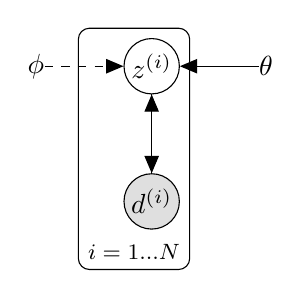
\begin{tikzpicture}[node distance = 1.5cm]
		
		
		\node[obs] (d) {$d^{(i)}$};
		
		\node[latent, above=of d] (z) {$z^{(i)}$};
		
		\node[const, right=of z] (th) {$\theta$} ;
		\node[const, left=of z] (ph) {$\phi$};
		
		
		\edge {z} {d};
		\edge {th} {z};
		\edge [dashed,bend left] {d} {z}
		\edge [dashed] {ph} {z}
		
		
		
		\plate {zd} {(z)(d)} {$i = 1...N$};
		
		\end{tikzpicture}
	\end{center}
	\caption{Graphical Model}
	\label{VAE}
\end{figure}


Discuss implications of plate difference? Discuss alternative approach with separate latent variables and/or noise for each word?\\ \\

\subsection{Application-specific choices}

For the encoder $q(z|x)$ and the decoder $p(x|z)$ we use fully connected neural networks. The prior $p(z)$ over the latent variables is a Multivariate Gaussian with diagonal covariance: $N(0,0.01*I)$. A smaller variance than the variance $I$, often used in VAE's, proved to be more effective. This is presumably because the KL divergence is less restrictive this way. 
\\
(need to show experiment for smaller KLD?)


The output of the decoder $p(x|z)$ is modeled as a Multinomial distribution. An obvious choice for count data such as bag-of-words data might also be a Poisson distribution. However, this also models document length, something we are not necessarily interested in.  

Even though we might not want to model document length, it might be informative for the topic. From that perspective, it makes sense not to normalize the input $X$. However, this requires the encoder to be able to generalize over different input scales, as opposed to working with normalized data. We therefore perform experiments with both approaches.

Discuss how interpretable the lower bound is (or later?). 

\subsection{Objective Function}

In a VAE, the log-likelihood of a data point i, $\mathbf{x}$, is written as a sum of the lower bound and the KL divergence term between the true posterior $p(z|x)$ and the approximation $q(z|x)$, with $\theta$ the parameters of the model:

\begin{align*}
\log p(\mathbf{x}^{(i)}) = D_{KL}(q(\mathbf{z}^{(i)}|\mathbf{x}^{(i)}) || p(\mathbf{z}|\mathbf{x}^{(i)})) + \mathcal{L}(\mathbf{\theta}, \phi)
\end{align*}

We optimize the lower bound on the log-likelihood: 

\begin{align}
%\mathcal{L}(\mathbf{\theta}, \phi; \mathbf{d}^{(i)}) = 
%\mathbf{E}_{q_\phi} (\mathbf{z}|\mathbf{d}^{(i)})}[-\log
%q_\ph	i (\mathbf{z}| \mathbf{d}^{(i)})+\log
%p_\theta(\mathbf{z}^{(i)}|\mathbf{d}^{(i)}]
\end{align}

which, using Bayes rule, we can express as:

\begin{align}
\mathcal{L}(\mathbf{\theta}, \phi; \mathbf{x}^{(i)}) = -D_{KL}(q_\phi (\mathbf{z}| \mathbf{x}^{(i)})||p_\theta (\mathbf{z})) + \mathbf{E}_{q_\phi(\mathbf{z}|\mathbf{x}^{(i)})}[\log p_\theta (\mathbf{x}^{(i)}|\mathbf{z})]
\end{align}



Still following Kingma and Welling \cite{kingma2013auto}, we can integrate the KL divergence analytically to obtain: \\


\begin{align}
- D_{KL}(q_\phi (\mathbf{z}| \mathbf{x}^{(i)}||p_\theta (\mathbf{z}| \mathbf{x}^{(i)})) = \frac{1}{2}\sum\limits_{j=1}^{J}\{1+\log \sigma_{\phi ,j}^2 - \mu_{\phi,j}^2 - \sigma_{\phi ,j}^2\}
\end{align}

Where the $\mathbf{\mu}_{\theta,j}$ and $\mathbf{\sigma}_{\theta,j}^2$ represent the $j$ -th mean and variance of the parametrized $q_\theta(\mathbf{z}|\mathbf{d})$.

An obvious choice for modeling the output distribution for count data would be Poisson. However, this also models the length of a document, which we do not expect to be very relevant for the topic. Therefore we use Multinomial probability for each word $x_n^{i}$ in document $d^{i}$. This way, we have that

\begin{align}
\log p_{\theta}(d^{(i)}|z^{(i)}) = 
\sum_{n=1}^N
\sum_{k=1}^K x_k^{(in)} \log (y_k^{(in)})
\end{align}
Where $k$ is the index of the output unit.\\


Using a SGVB estimator, our final objective function consists of the negative KL divergence and the reconstruction error:

\begin{align}
\mathcal{L}(\mathbf{\theta}, \phi; \mathbf{d}^{(i)}) = \frac{1}{2}\sum\limits_{j=1}^{J}\{1+\log \sigma_{\phi ,j}^2 - \mu_{\phi,j}^2 - \sigma_{\phi ,j}^2\} 
+ \sum_{n=1}^N
\sum_{k=1}^K x_k^{(in)} \log (y_k^{(in)})
\end{align}

\subsection{old derivation of objective function}

In a VAE, the log-likelihood of a data point i, $\mathbf{x}$, is written as a sum of the lower bound and the KL divergence term between the true posterior $p(z|x)$ and the approximation $q(z|x)$, with $\theta$ the parameters of the model:

\begin{align*}
\log p(\mathbf{x}^{(i)}) = D_{KL}(q(\mathbf{z}^{(i)}|\mathbf{x}^{(i)}) || p(\mathbf{z}|\mathbf{x}^{(i)})) + \mathcal{L}(\mathbf{\theta}, \phi)
\end{align*}

We optimize the lower bound on the log-likelihood: 

\begin{align}
%\mathcal{L}(\mathbf{\theta}, \phi; \mathbf{d}^{(i)}) = 
%\mathbf{E}_{q_\phi} (\mathbf{z}|\mathbf{d}^{(i)})}[-\log
%q_\ph	i (\mathbf{z}| \mathbf{d}^{(i)})+\log
%p_\theta(\mathbf{z}^{(i)}|\mathbf{d}^{(i)}]
\end{align}

which, using Bayes rule, we can express as:

\begin{align}
\mathcal{L}(\mathbf{\theta}, \phi; \mathbf{x}^{(i)}) = -D_{KL}(q_\phi (\mathbf{z}| \mathbf{x}^{(i)})||p_\theta (\mathbf{z})) + \mathbf{E}_{q_\phi(\mathbf{z}|\mathbf{x}^{(i)})}[\log p_\theta (\mathbf{x}^{(i)}|\mathbf{z})]
\end{align}



Still following Kingma and Welling \cite{kingma2013auto}, we can integrate the KL divergence analytically to obtain: \\


\begin{align}
- D_{KL}(q_\phi (\mathbf{z}| \mathbf{x}^{(i)}||p_\theta (\mathbf{z}| \mathbf{x}^{(i)})) = \frac{1}{2}\sum\limits_{j=1}^{J}\{1+\log \sigma_{\phi ,j}^2 - \mu_{\phi,j}^2 - \sigma_{\phi ,j}^2\}
\end{align}

Where the $\mathbf{\mu}_{\theta,j}$ and $\mathbf{\sigma}_{\theta,j}^2$ represent the $j$ -th mean and variance of the parametrized $q_\theta(\mathbf{z}|\mathbf{d})$.

An obvious choice for modeling the output distribution for count data would be Poisson. However, this also models the length of a document, which we do not expect to be very relevant for the topic. Therefore we use Multinomial probability for each word $x_n^{i}$ in document $d^{i}$. This way, we have that

\begin{align}
\log p_{\theta}(d^{(i)}|z^{(i)}) = 
\sum_{n=1}^N
\sum_{k=1}^K x_k^{(in)} \log (y_k^{(in)})
\end{align}
Where $k$ is the index of the output unit.\\


Using a SGVB estimator, our final objective function consists of the negative KL divergence and the reconstruction error:

\begin{align}
\mathcal{L}(\mathbf{\theta}, \phi; \mathbf{d}^{(i)}) = \frac{1}{2}\sum\limits_{j=1}^{J}\{1+\log \sigma_{\phi ,j}^2 - \mu_{\phi,j}^2 - \sigma_{\phi ,j}^2\} 
+ \sum_{n=1}^N
\sum_{k=1}^K x_k^{(in)} \log (y_k^{(in)})
\end{align}

\bibliography{ref}
\end{document}